%%%%%%%%%%%%%%%%%%%%%%%%%%%%%%%%%%%%%%%%%
% baposter Landscape Poster
% LaTeX Template
% Version 1.0 (11/06/13)
%
% baposter Class Created by:
% Brian Amberg (baposter@brian-amberg.de)
%
% This template has been downloaded from:
% http://www.LaTeXTemplates.com
%
% License:
% CC BY-NC-SA 3.0 (http://creativecommons.org/licenses/by-nc-sa/3.0/)
%
%%%%%%%%%%%%%%%%%%%%%%%%%%%%%%%%%%%%%%%%%

%----------------------------------------------------------------------------------------
%	PACKAGES AND OTHER DOCUMENT CONFIGURATIONS
%----------------------------------------------------------------------------------------

\documentclass[landscape,a0paper,fontscale=0.400]{baposter} % Adjust the font scale/size here

\usepackage{graphicx} % Required for including images
\graphicspath{{figures/}} % Directory in which figures are stored

\usepackage{amsmath} % For typesetting math
\usepackage{amssymb} % Adds new symbols to be used in math mode

\usepackage[backend=biber]{biblatex}
\bibliography{sample} 

\usepackage{wrapfig} % Allows text embedding of figures
\usepackage{booktabs} % Top and bottom rules for tables
\usepackage{enumitem} % Used to reduce itemize/enumerate spacing
\usepackage{palatino} % Use the Palatino font
\usepackage[font=small,labelfont=bf]{caption} % Required for specifying captions to tables and figures

\usepackage{multicol} % Required for multiple columns
\setlength{\columnsep}{1.5em} % Slightly increase the space between columns
\setlength{\columnseprule}{0mm} % No horizontal rule between columns

\usepackage{tikz, tikz-3dplot, standalone} % Required for embedding tikz
\usetikzlibrary{quotes, angles} % more tikz stuff
\usetikzlibrary{shapes,arrows} % Tikz libraries required for the flow chart in the template

\newcommand{\compresslist}{ % Define a command to reduce spacing within itemize/enumerate environments, this is used right after \begin{itemize} or \begin{enumerate}
\setlength{\itemsep}{1pt}
\setlength{\parskip}{0pt}
\setlength{\parsep}{0pt}
}

%Pre-defined lightblue \definecolor{lightblue}{rgb}{0.145,0.6666,1} % Defines the color used for content box headers
%Original lightblue \definecolor{lightblue}{RGB}{33,147,253}
\definecolor{lightblue}{RGB}{122,221,255}
% Original myblue \definecolor{myblue}{RGB}{0,107,255}
\definecolor{myblue}{RGB}{33,147,253}

\begin{document}

\begin{poster}
{
headerborder=closed, % Adds a border around the header of content boxes
colspacing=1em, % Column spacing
bgColorOne=white, % Background color for the gradient on the left side of the poster
bgColorTwo=white, % Background color for the gradient on the right side of the poster
borderColor=lightblue, % Border color
headerColorOne=myblue, % Background color for the header in the content boxes (left side)
headerColorTwo=lightblue, % Background color for the header in the content boxes (right side)
headerFontColor=white, % Text color for the header text in the content boxes
boxColorOne=white, % Background color of the content boxes
textborder=roundedleft, % Format of the border around content boxes, can be: none, bars, coils, triangles, rectangle, rounded, roundedsmall, roundedright or faded
eyecatcher=true, % Set to false for ignoring the left logo in the title and move the title left
headerheight=0.1\textheight, % Height of the header
headershape=roundedright, % Specify the rounded corner in the content box headers, can be: rectangle, small-rounded, roundedright, roundedleft or rounded
headerfont=\Large\bf\textsc, % Large, bold and sans serif font in the headers of content boxes
%textfont={\setlength{\parindent}{1.5em}}, % Uncomment for paragraph indentation
linewidth=2pt % Width of the border lines around content boxes
}
%----------------------------------------------------------------------------------------
%	TITLE SECTION 
%----------------------------------------------------------------------------------------
%
{
\includegraphics[height=8.5em]{logo2}} % First university/lab logo on the left
{\bf\textsc{\textcolor{black}{An Analysis of Radio Meteor Detection}}\vspace{0.5em}} % Poster title
{\textsc{\{ \textcolor{blue}{Charles Powell} \} \hspace{12pt} \textcolor{blue}{Exeter Mathematics School \& Norman Lockyer Observatory}}} % Author names and institution
{
\includegraphics[height=7em]{nlo}} % Second university/lab logo on the right

%----------------------------------------------------------------------------------------
%	OVERVIEW
%----------------------------------------------------------------------------------------

\headerbox{Overview}{name=objectives,column=0,row=0}{
\begin{wrapfigure}{r}{0.3\linewidth}
	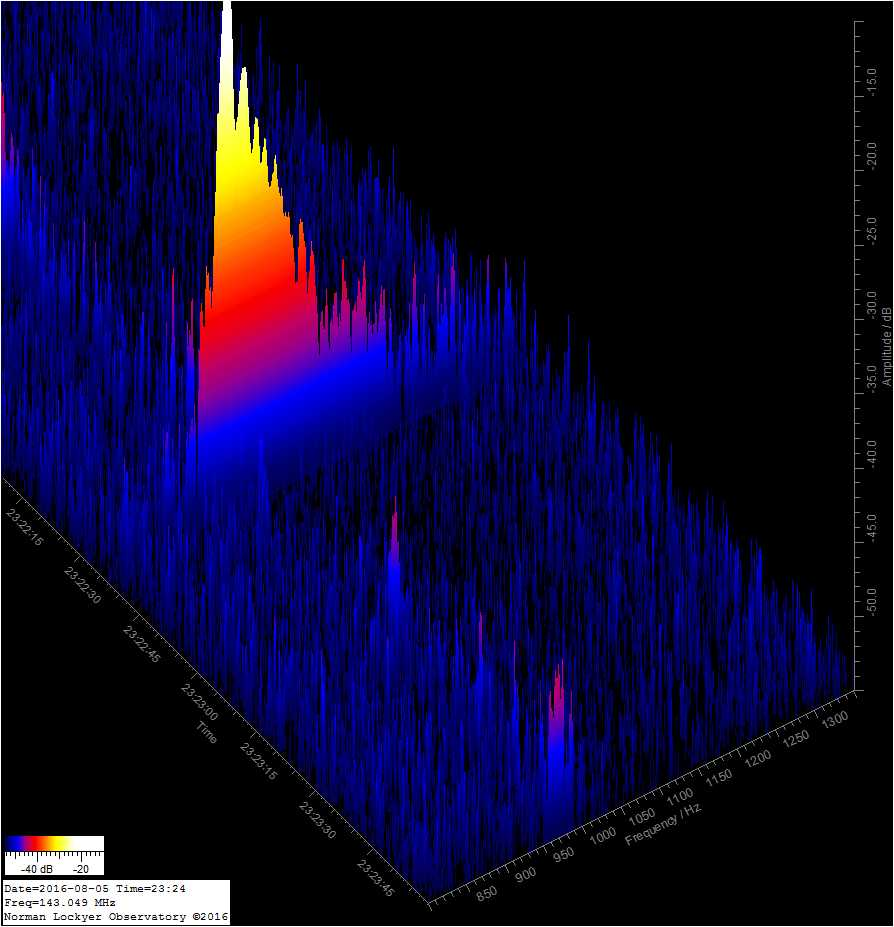
\includegraphics[width=\linewidth]{3D}
	\caption{3D Waterfall Plot \label{fig:waterfall}}
\end{wrapfigure}
Meteors have three stages to their lives. They start as rocky or metallic bodies in space, where they are known as meteoroids. Once a meteoroid enters the Earth's atmosphere, it is heated by friction and this extreme heat ionises the air around the meteor, creating a visible streak which is commonly known as a `shooting star'. If any of the meteor makes it to the ground, it becomes a meteorite. The ionised air around the meteor reflects radio waves. This is the fundamental principle behind radio meteor detection.
The detection starts with a transmitting antenna sending out a signal into the upper atmosphere. The signal reflects off of the ionised trail left by the meteor, and is received by another antenna. The way this signal is visualised is typically as a `waterfall' plot (figure~\ref{fig:waterfall}). Alternatively, software is used to count meteors from the signal.

\vspace{0.3em} % When there are two boxes, some whitespace may need to be added if the one on the right has more content
}

%----------------------------------------------------------------------------------------
%	IMAGE ANALYSIS
%----------------------------------------------------------------------------------------

\headerbox{Detection By Image Analysis}{name=introduction,column=1,row=0,bottomaligned=objectives}{
\begin{wrapfigure}{r}{0.4\linewidth}
	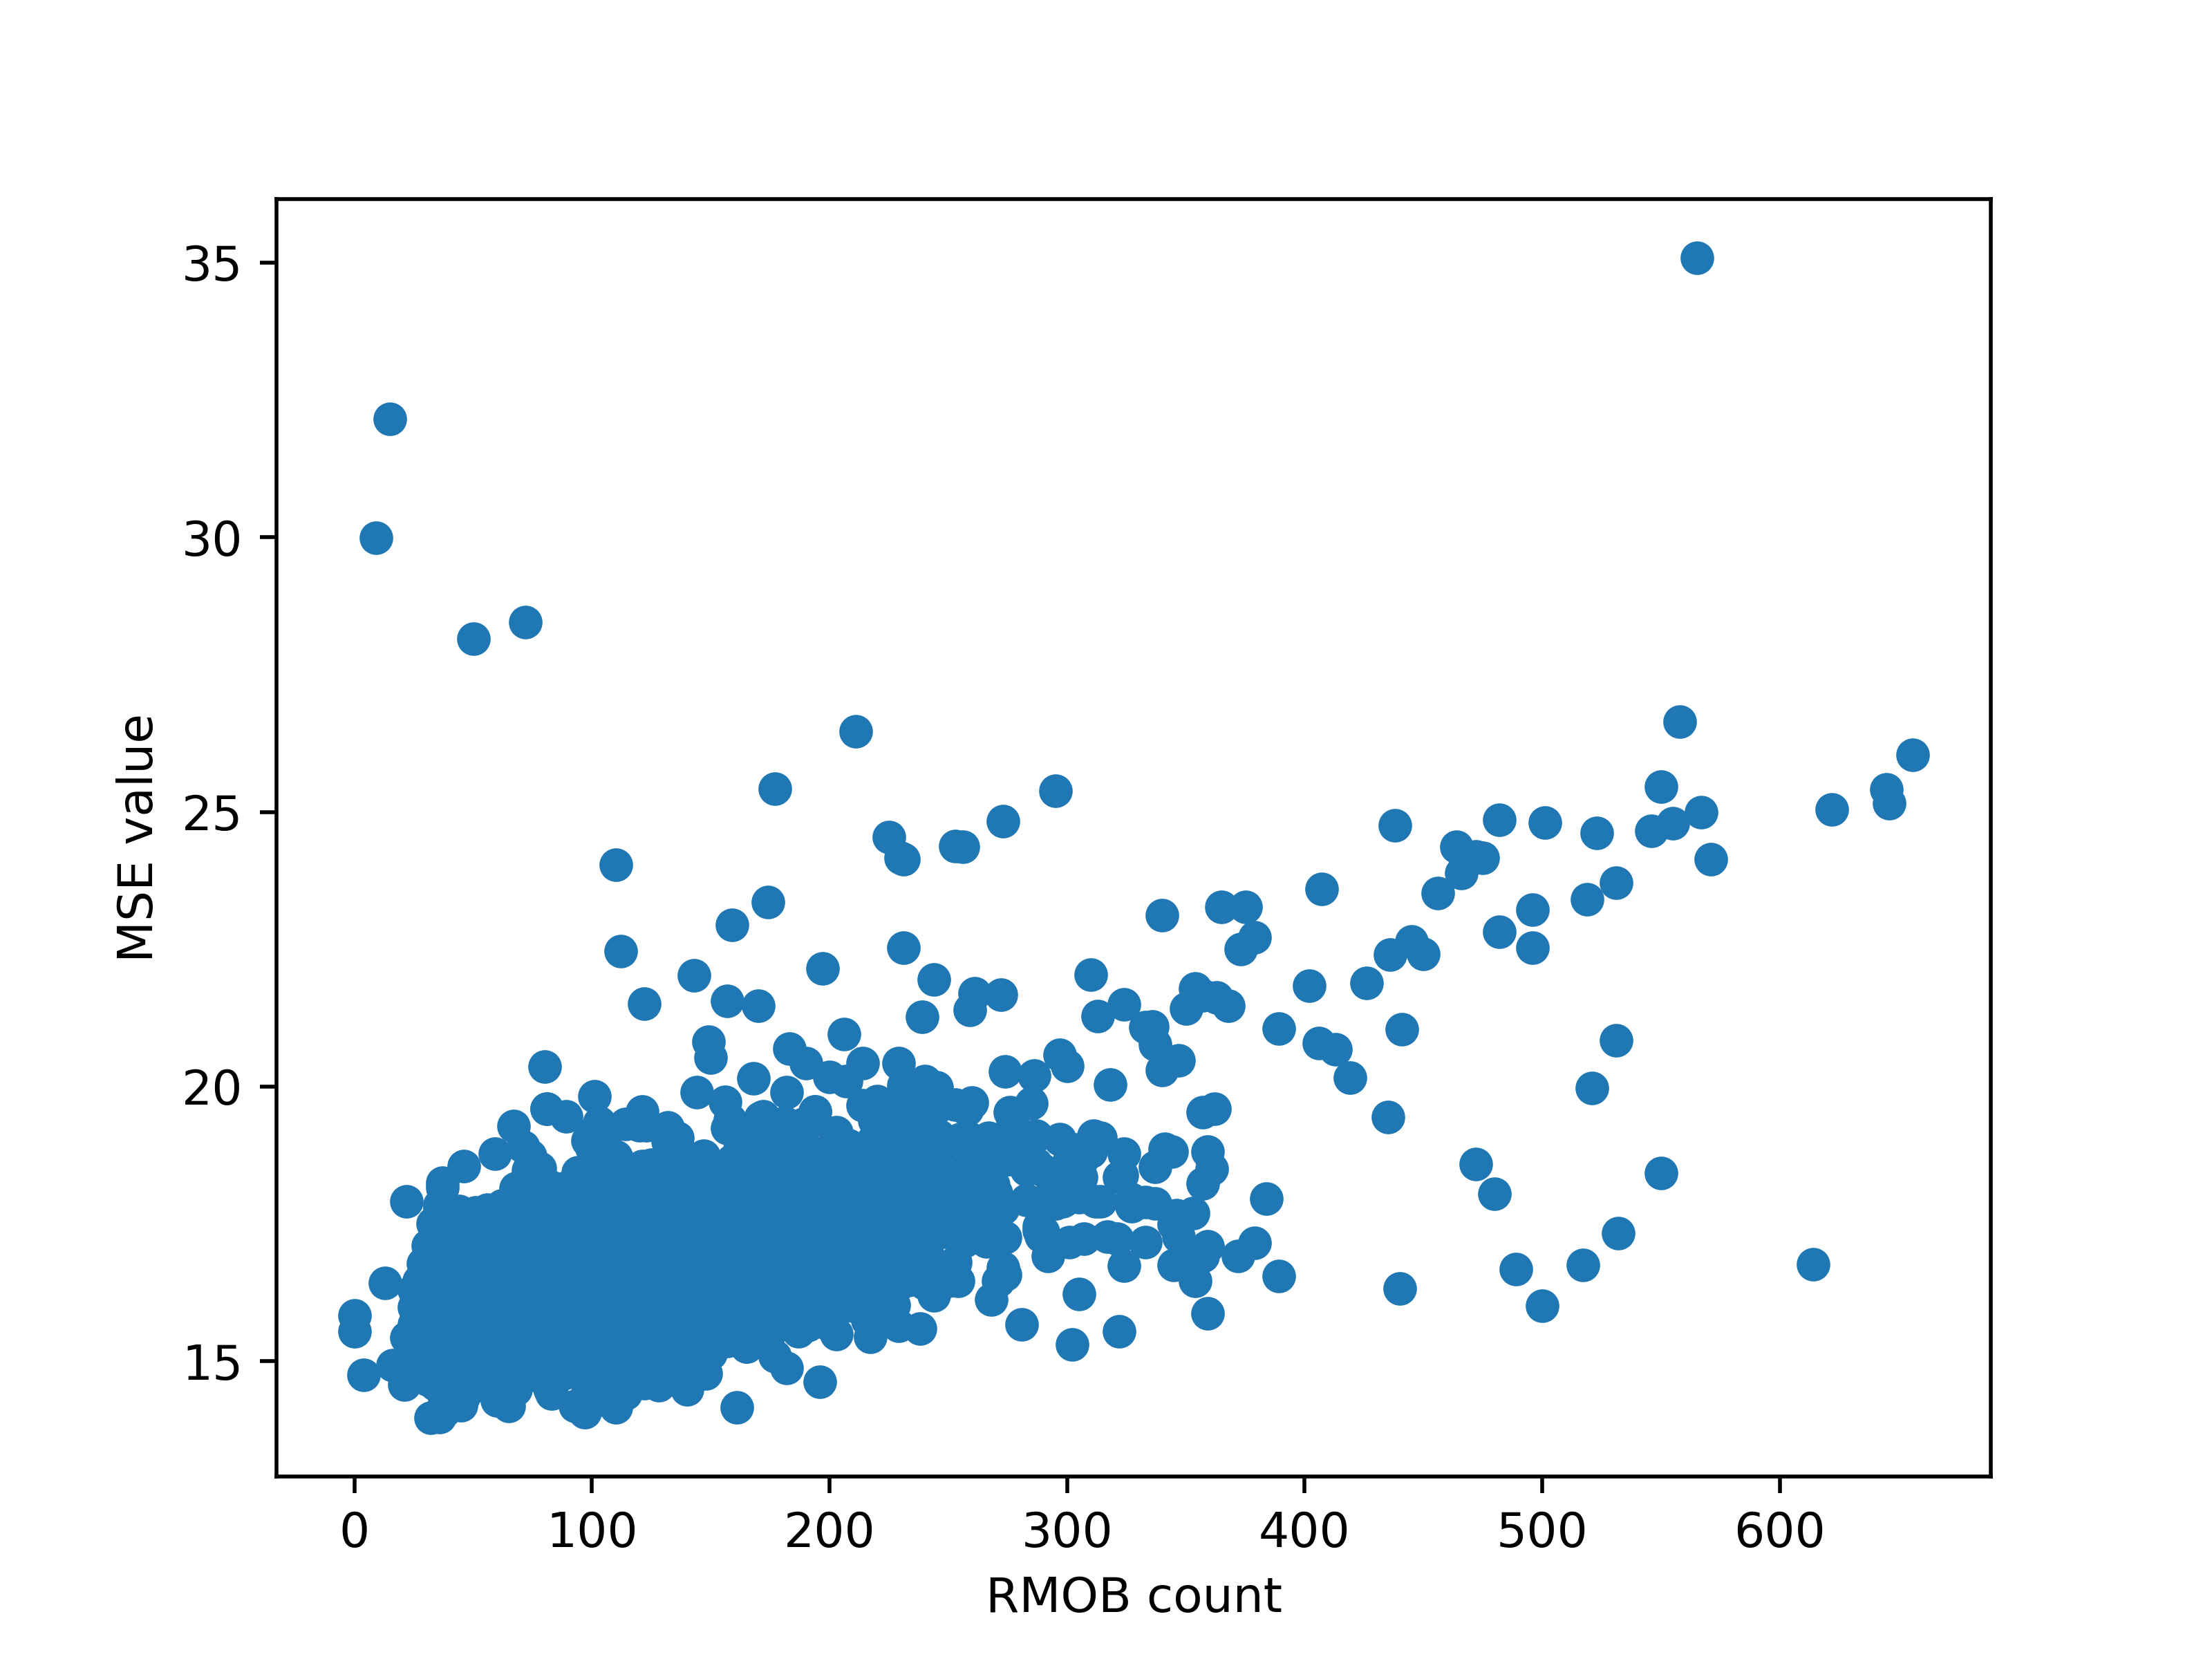
\includegraphics[width=\linewidth]{after}
	\caption{RMS difference vs. RMOB count \label{fig:rms}}
\end{wrapfigure}
The idea of detection by image analysis is to identify areas of the image with a distinct signal, which are considered to be meteors (note the large yellow area in figure~\ref{fig:waterfall}). Root mean square difference is a method of identifying distinct signals, which works by calculating a measure of the difference between corresponding pixels in two images: the signal image, and a `baseline' image.
In order to test how well this method works, I tested for correlation with a set of data that is known to work: hourly detection counts (from RMOB), as used in my other studies. The result is a correlation coefficient (using Pearson's Moment) of $r = 0.6165$, with a p-value of $p=4.05\cdot10^{-214}$, suggesting a good correlation between the two data sets (figure~\ref{fig:rms}).

}

%----------------------------------------------------------------------------------------
%	TEMPORAL, SPATIAL AND ANTENNA TYPE VARIATION
%----------------------------------------------------------------------------------------

\headerbox{Temporal, Spatial \& Antenna Type Variation}{name=results,column=2,span=2,row=0}{

\begin{multicols}{3}
{\large \bf Temporal Variation\\}

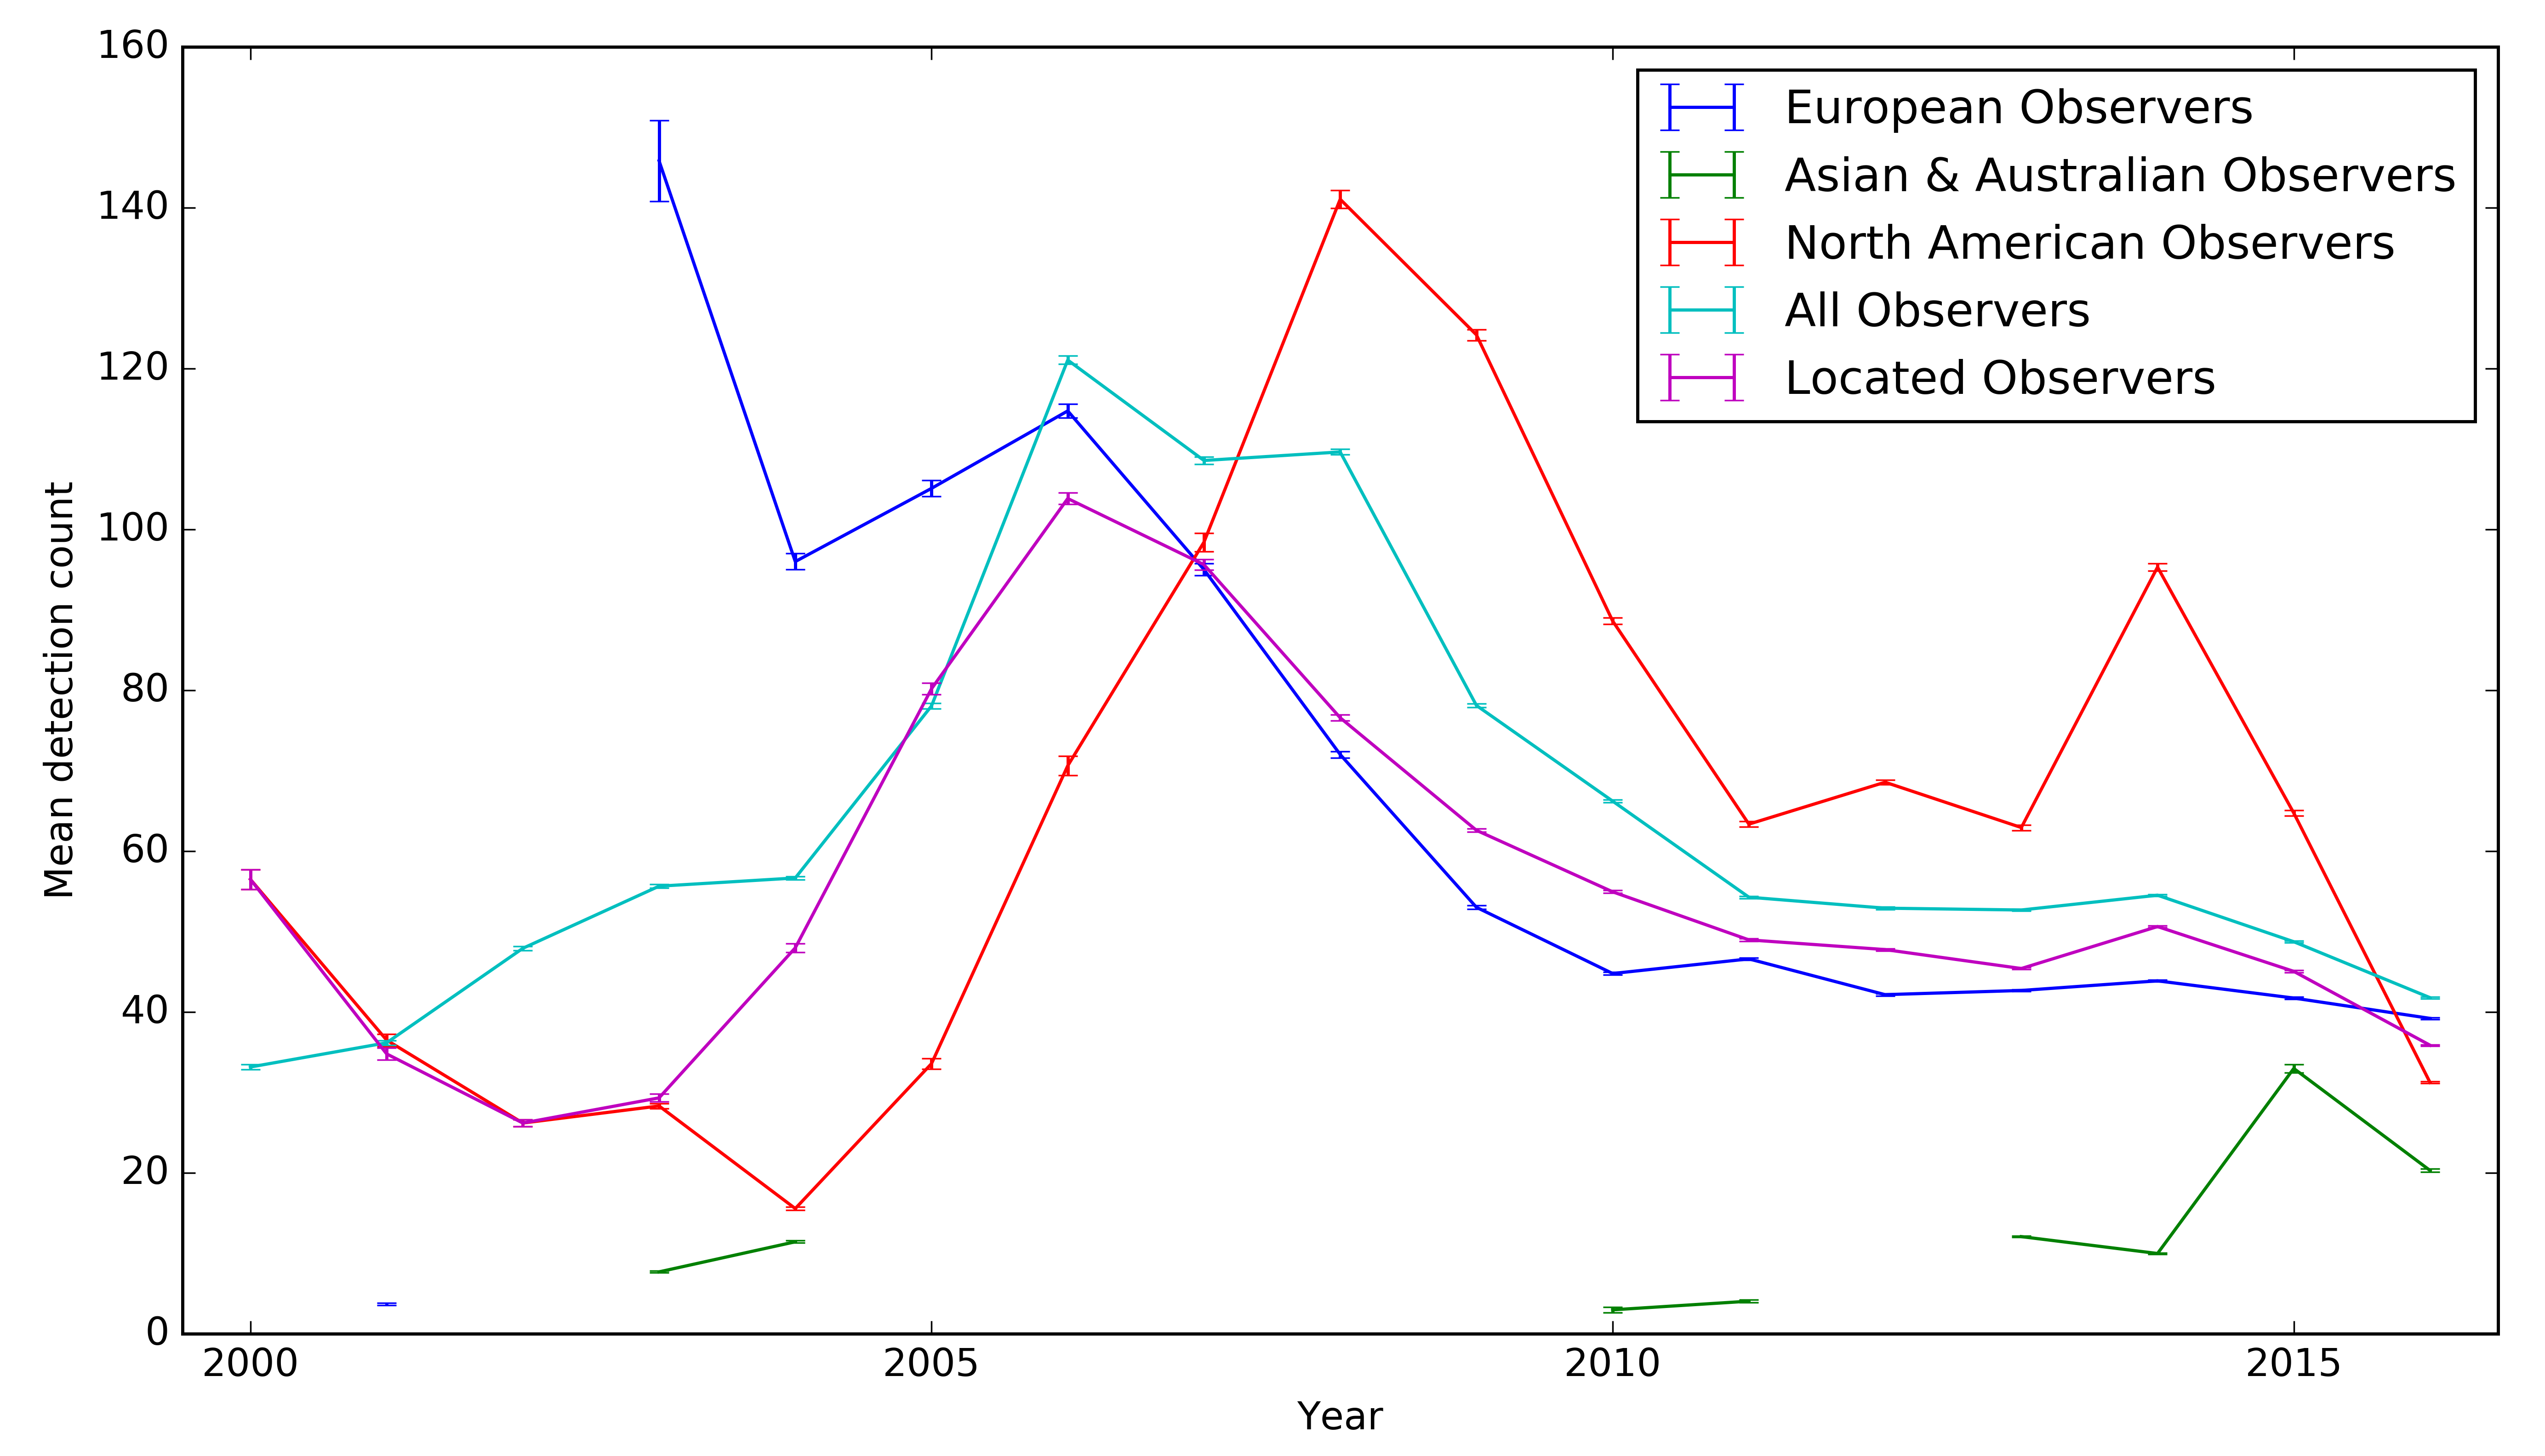
\includegraphics[width=\linewidth]{Ycombined}
\captionof{figure}{Variation in mean hourly detection count since 2000 by year \label{fig:years}}

\vspace{1em}

I have analysed the variation of detection counts and other descriptive characteristics of the data over time. There is a significant increase in detection counts between 2005 and 2011 (see figure~\ref{fig:years}), which links to the minimum of the solar cycle. This indicates that the activity of the Sun (and most likely the solar wind) prevents some radio meteor detection, since when the solar wind has a greater intensity, there is a greater electron density in the upper atmosphere, influencing radio signals.

\columnbreak

\begin{center}
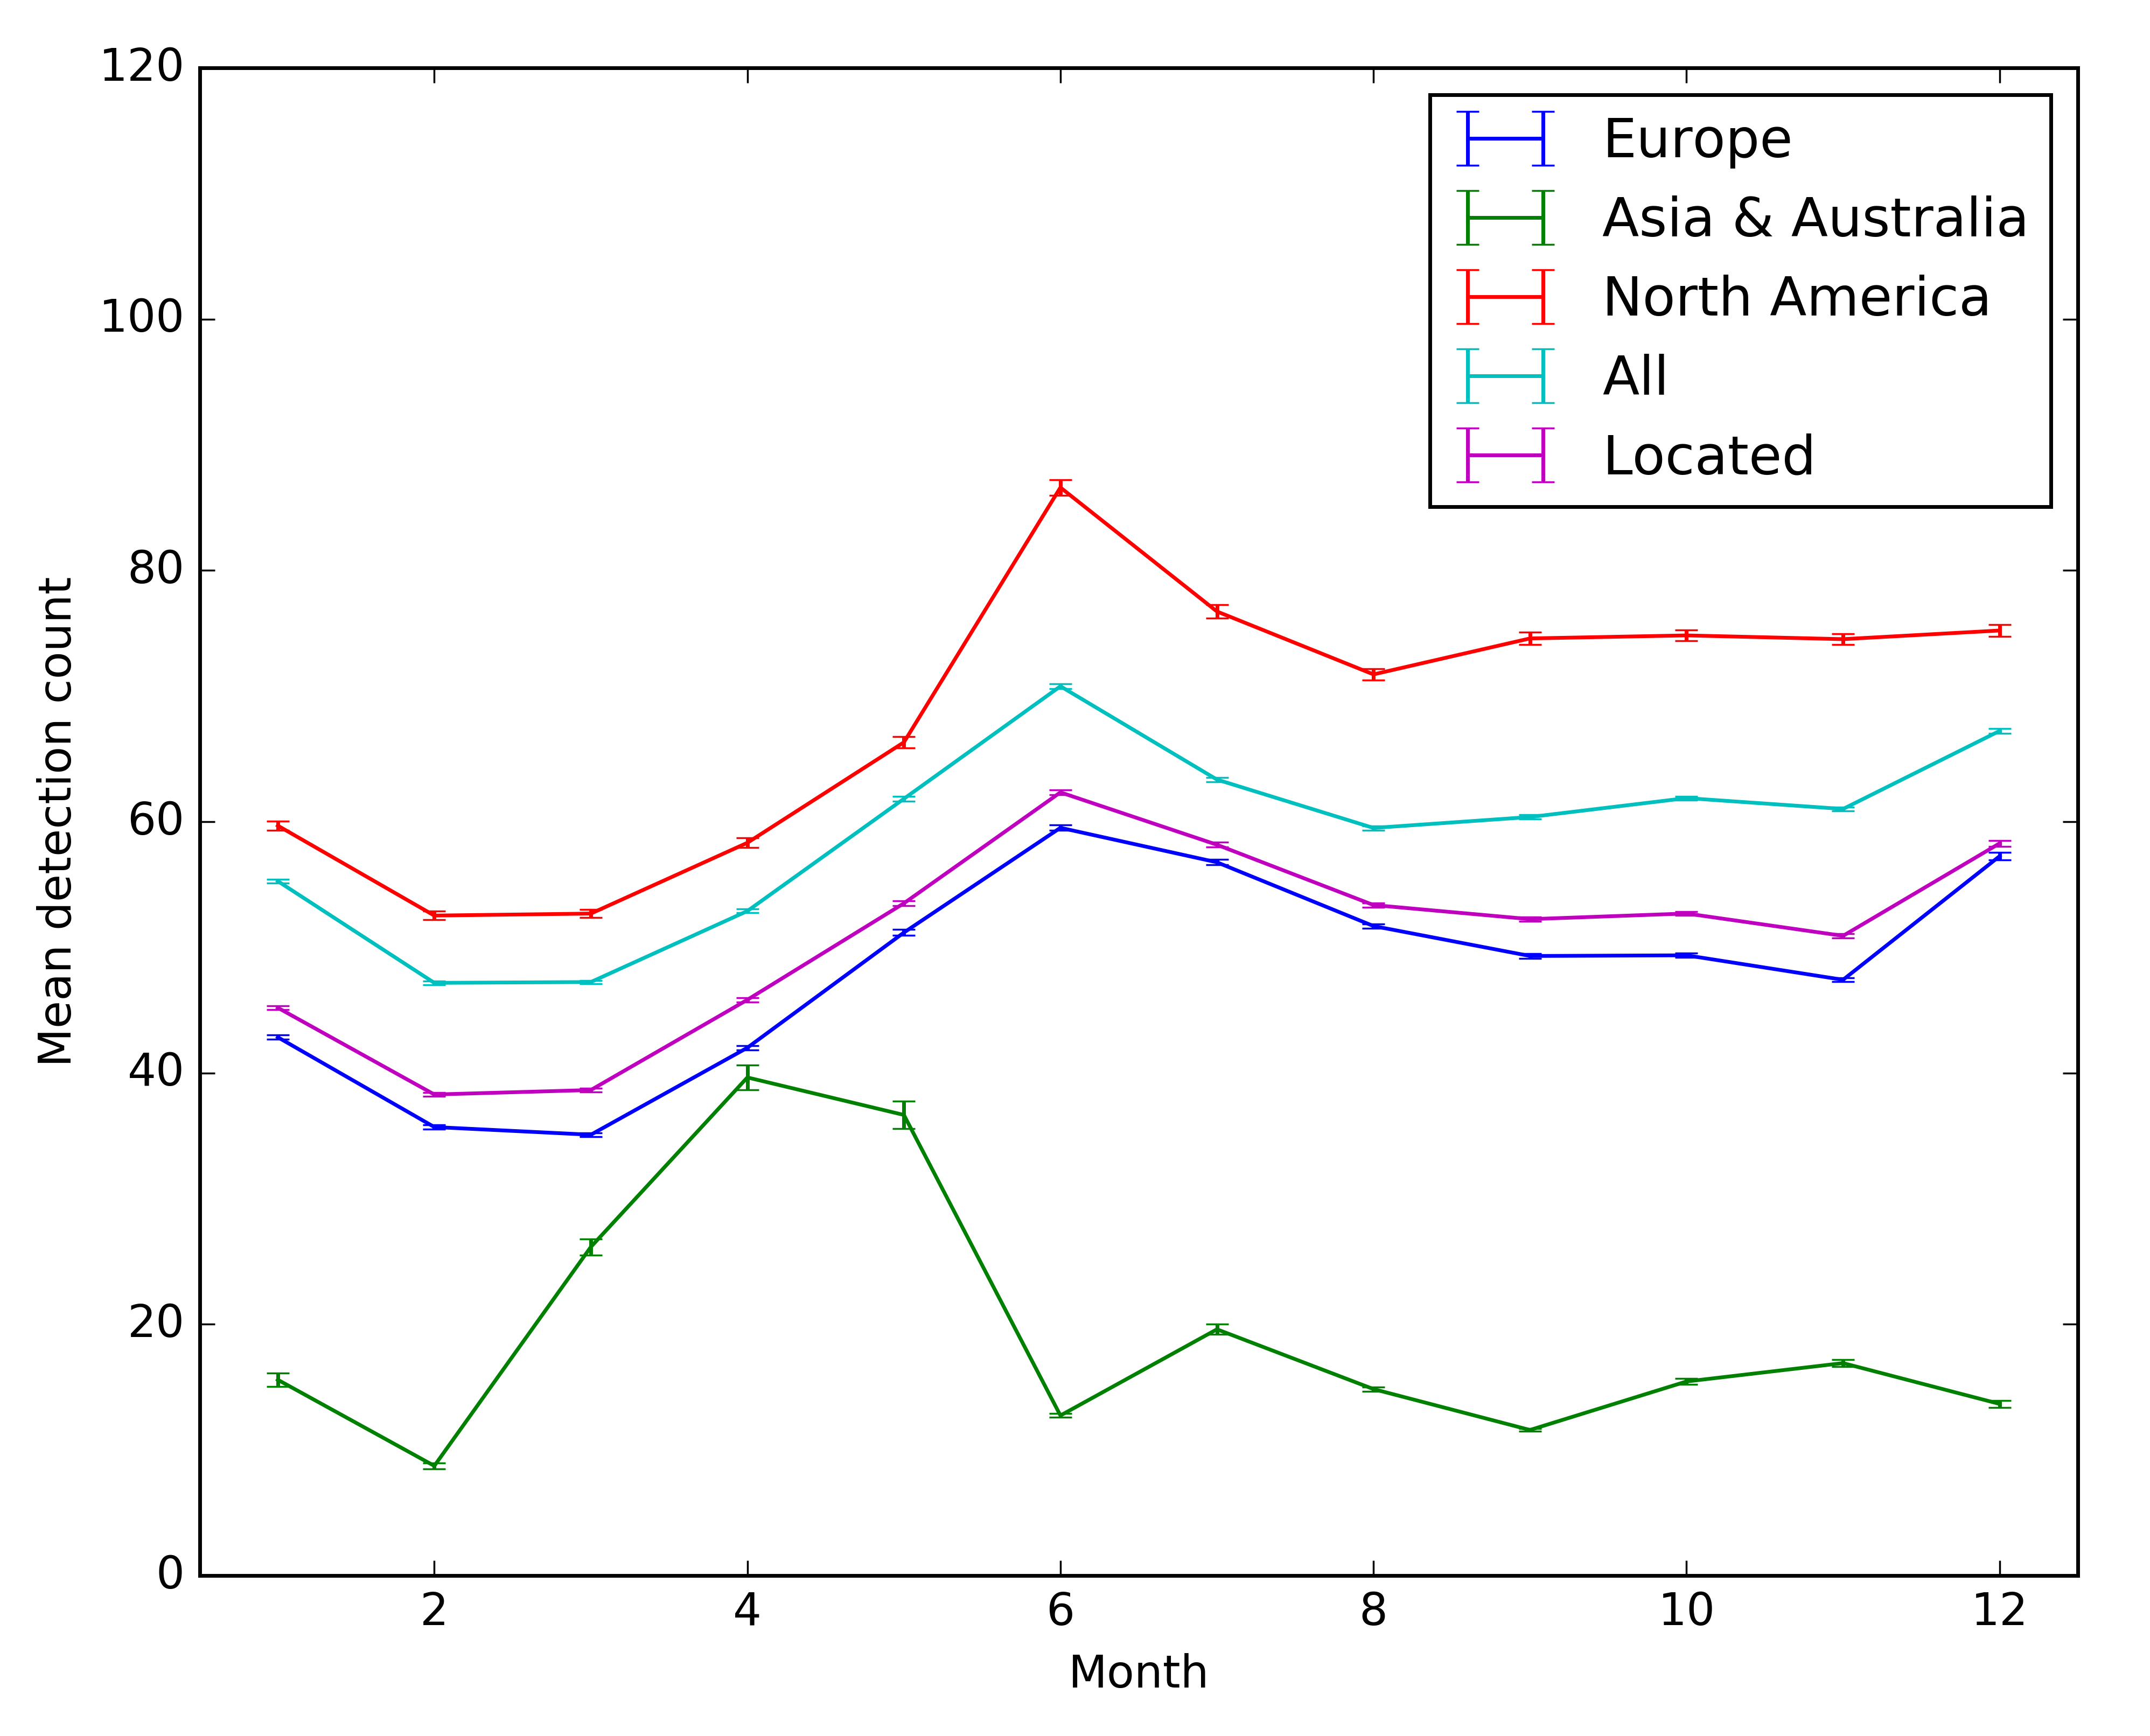
\includegraphics[width=0.8\linewidth]{Mcombined}
\end{center}
\captionof{figure}{Variation in mean hourly detection count over a year \label{fig:annual}}
\vspace{1em}

The results (figure~\ref{fig:annual}) also show an increase in detection counts in the middle of the year, which persists for the rest of the year. This could be due to an increased number of meteor showers, or other effects which I have not studied. I have found little variation of detection counts during each month, as expected, since there are few effects that vary on a monthly basis. With a 1\% significance level, there is no difference between daytime and night-time detection rates.

\vfill\null
\columnbreak
%------------------------------------------------

{\large \bf Spatial Variation\\}
Most data characteristics do not correlate well with latitude or longitude, implying the location where a detection takes place has little impact on the resulting detections. As expected, there is a correlation between longitude and peak hour of diurnal shift. Other studies \cite{latitudes} have noted a correlation between latitude and the intensity of diurnal shift, though my results do not clearly support this. The implication of these findings is that, across the globe, the quality and quantity of radio meteor detection doesn't change, which in itself suggests a uniform distribution of sporadic meteors in space. \\

%------------------------------------------------

{\large \bf Variation by antenna type\\}
Overall, there is little variation between antenna types, and a large degree of variation between observers with the same antennas, implying that the choice has little effect on the results of radio meteor detection. However, J-pole, log periodic and turnstile antennas appear to produce the most extreme results. However, this is likely due to anomalous readings. \\
\end{multicols}
}

%----------------------------------------------------------------------------------------
%	REFERENCES
%----------------------------------------------------------------------------------------

\headerbox{References}{name=references,column=0,above=bottom}{

\renewcommand{\section}[2]{\vskip 0.05em} % Get rid of the default "References" section title
\small{ % Reduce the font size in this block
\printbibliography% Use sample.bib as the bibliography file
}}

%----------------------------------------------------------------------------------------
%	FUTURE WORK
%----------------------------------------------------------------------------------------

\headerbox{Future Work}{name=futureresearch,column=1,span=2,aligned=references,above=bottom}{ % This block is as tall as the references block

\begin{multicols}{2}
	
For many results, there is yet a conclusion to be made. There are many variables that influence radio meteor detection in conjunction with one another, making isolation of a variable and consequent analysis difficult. A larger set of data, with a more uniform coverage of the globe, is the aim for the future, as well as extensions of the analyses in order to refine and validate conclusions. 

\end{multicols}
}

%----------------------------------------------------------------------------------------
%	ACKNOWLEDGEMENTS
%----------------------------------------------------------------------------------------

\headerbox{Acknowledgements}{name=contact,column=3,aligned=references,above=bottom}{ % This block is as tall as the references block

I am indebted to the RMOB organization \cite{rmob} for permission to use their data. Credit is also due to the Norman Lockyer Observatory, where I have worked on this project, utilised my detection method, and sourced data.

}

%----------------------------------------------------------------------------------------
%	DIURNAL SHIFT
%----------------------------------------------------------------------------------------

\headerbox{Diurnal Variation of Meteor Flux}{name=conclusion,column=2,span=2,row=0,below=results,above=references}{

\begin{multicols}{2}
	
\begin{wrapfigure}[12]{r}{0.45\linewidth}
	\centering
	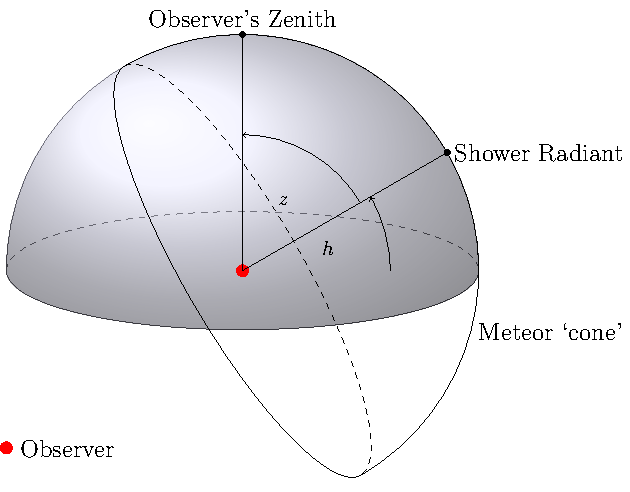
\includegraphics[width=\linewidth]{diagram}
	\caption{Diagram of diurnal shift model \label{fig:diagram}}
\end{wrapfigure}

Diurnal shift is an observed increase and decrease in detection counts over a day. Some models explain this as the Earth `intercepting more sporadic meteors at Sunrise than Sunset', though this is inconsistent. I propose that the incident velocity, added to Earth's orbital velocity at Sunrise ($\sim 6$am observer's local time), results in a higher intercept velocity, meaning more detections occur since more meteors reach the atmosphere (see figure~\ref{fig:diagram}).\\

\begin{wrapfigure}[15]{l}{0.65\linewidth}
	\centering
	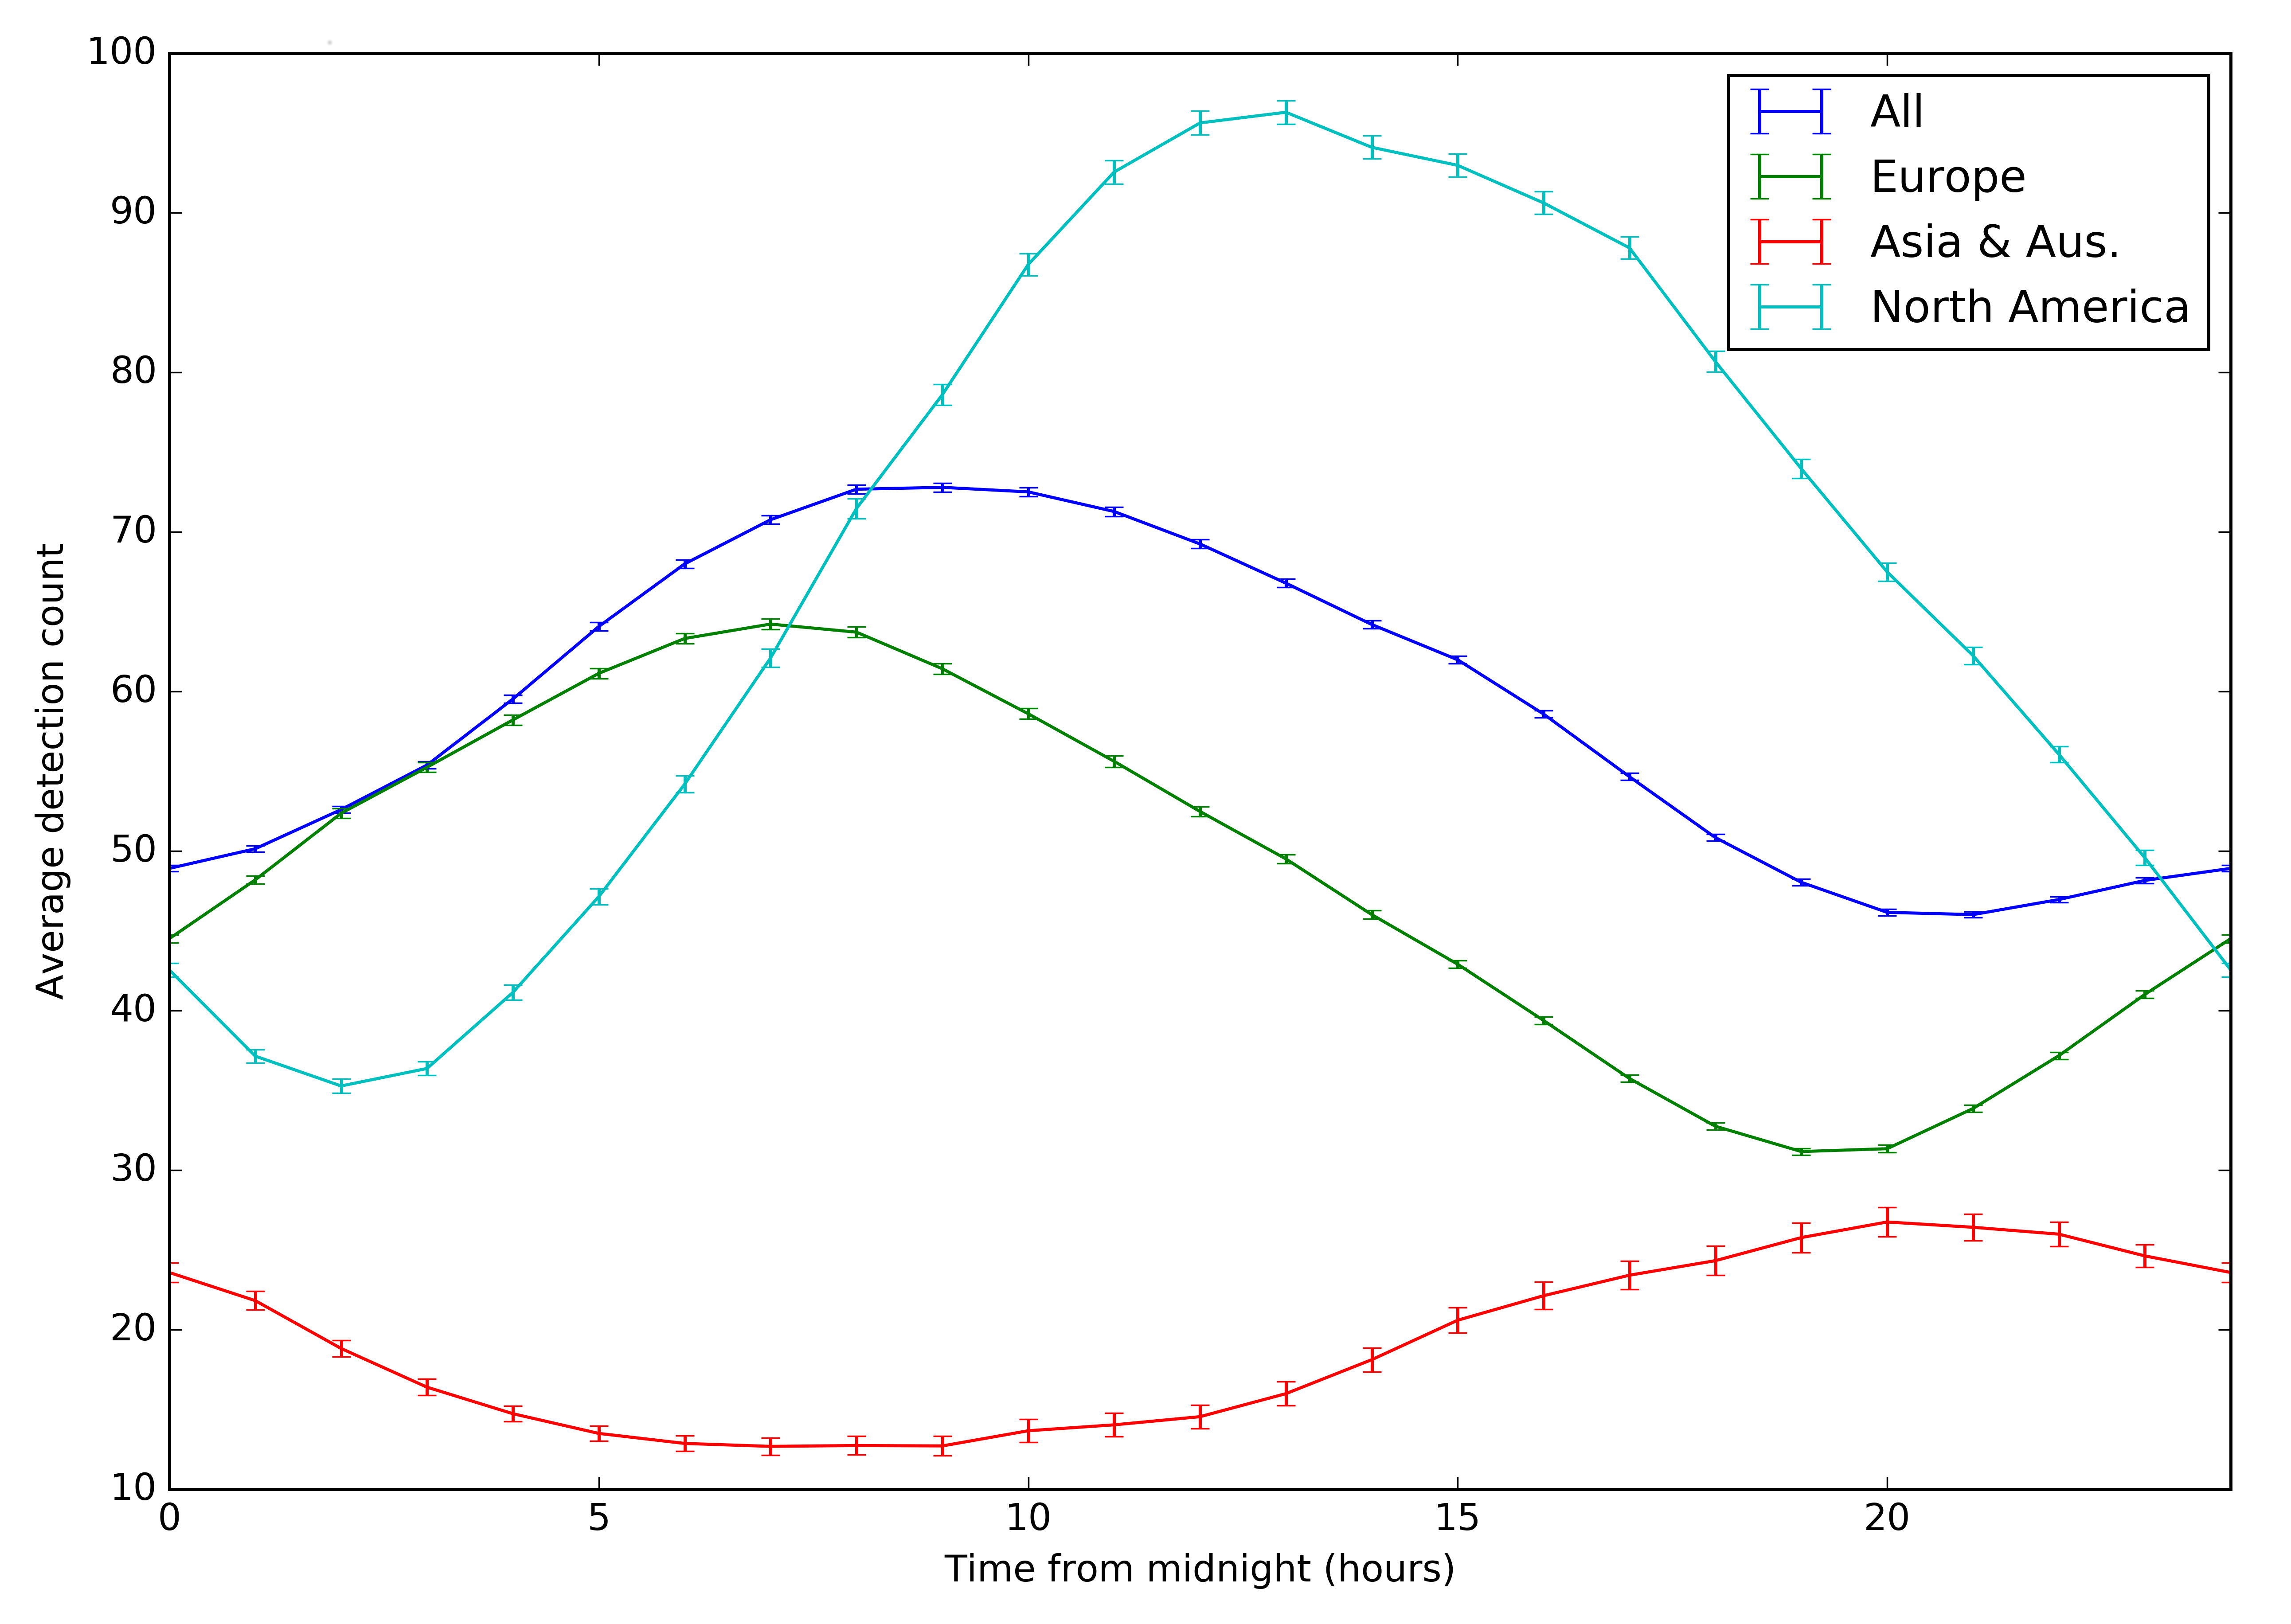
\includegraphics[width=\linewidth]{all_shifts}
	\caption{Diurnal shifts for various locations
		\label{fig:shifts}}
\end{wrapfigure}

A sinusoidal function fits the mean diurnal shift of each category well (see figure~\ref{fig:shifts}), indicating that my model, which is based around a cosine function, is consistent. It is apparent that the diurnal shift occurs worldwide, and varies in amplitude between locations, supporting other studies. \\

\vspace{2em}
\vfill\null
\columnbreak

{\large \bf Spatial variation of diurnal shift\\}

\begin{wrapfigure}{r}{0.5\linewidth}
	\centering
	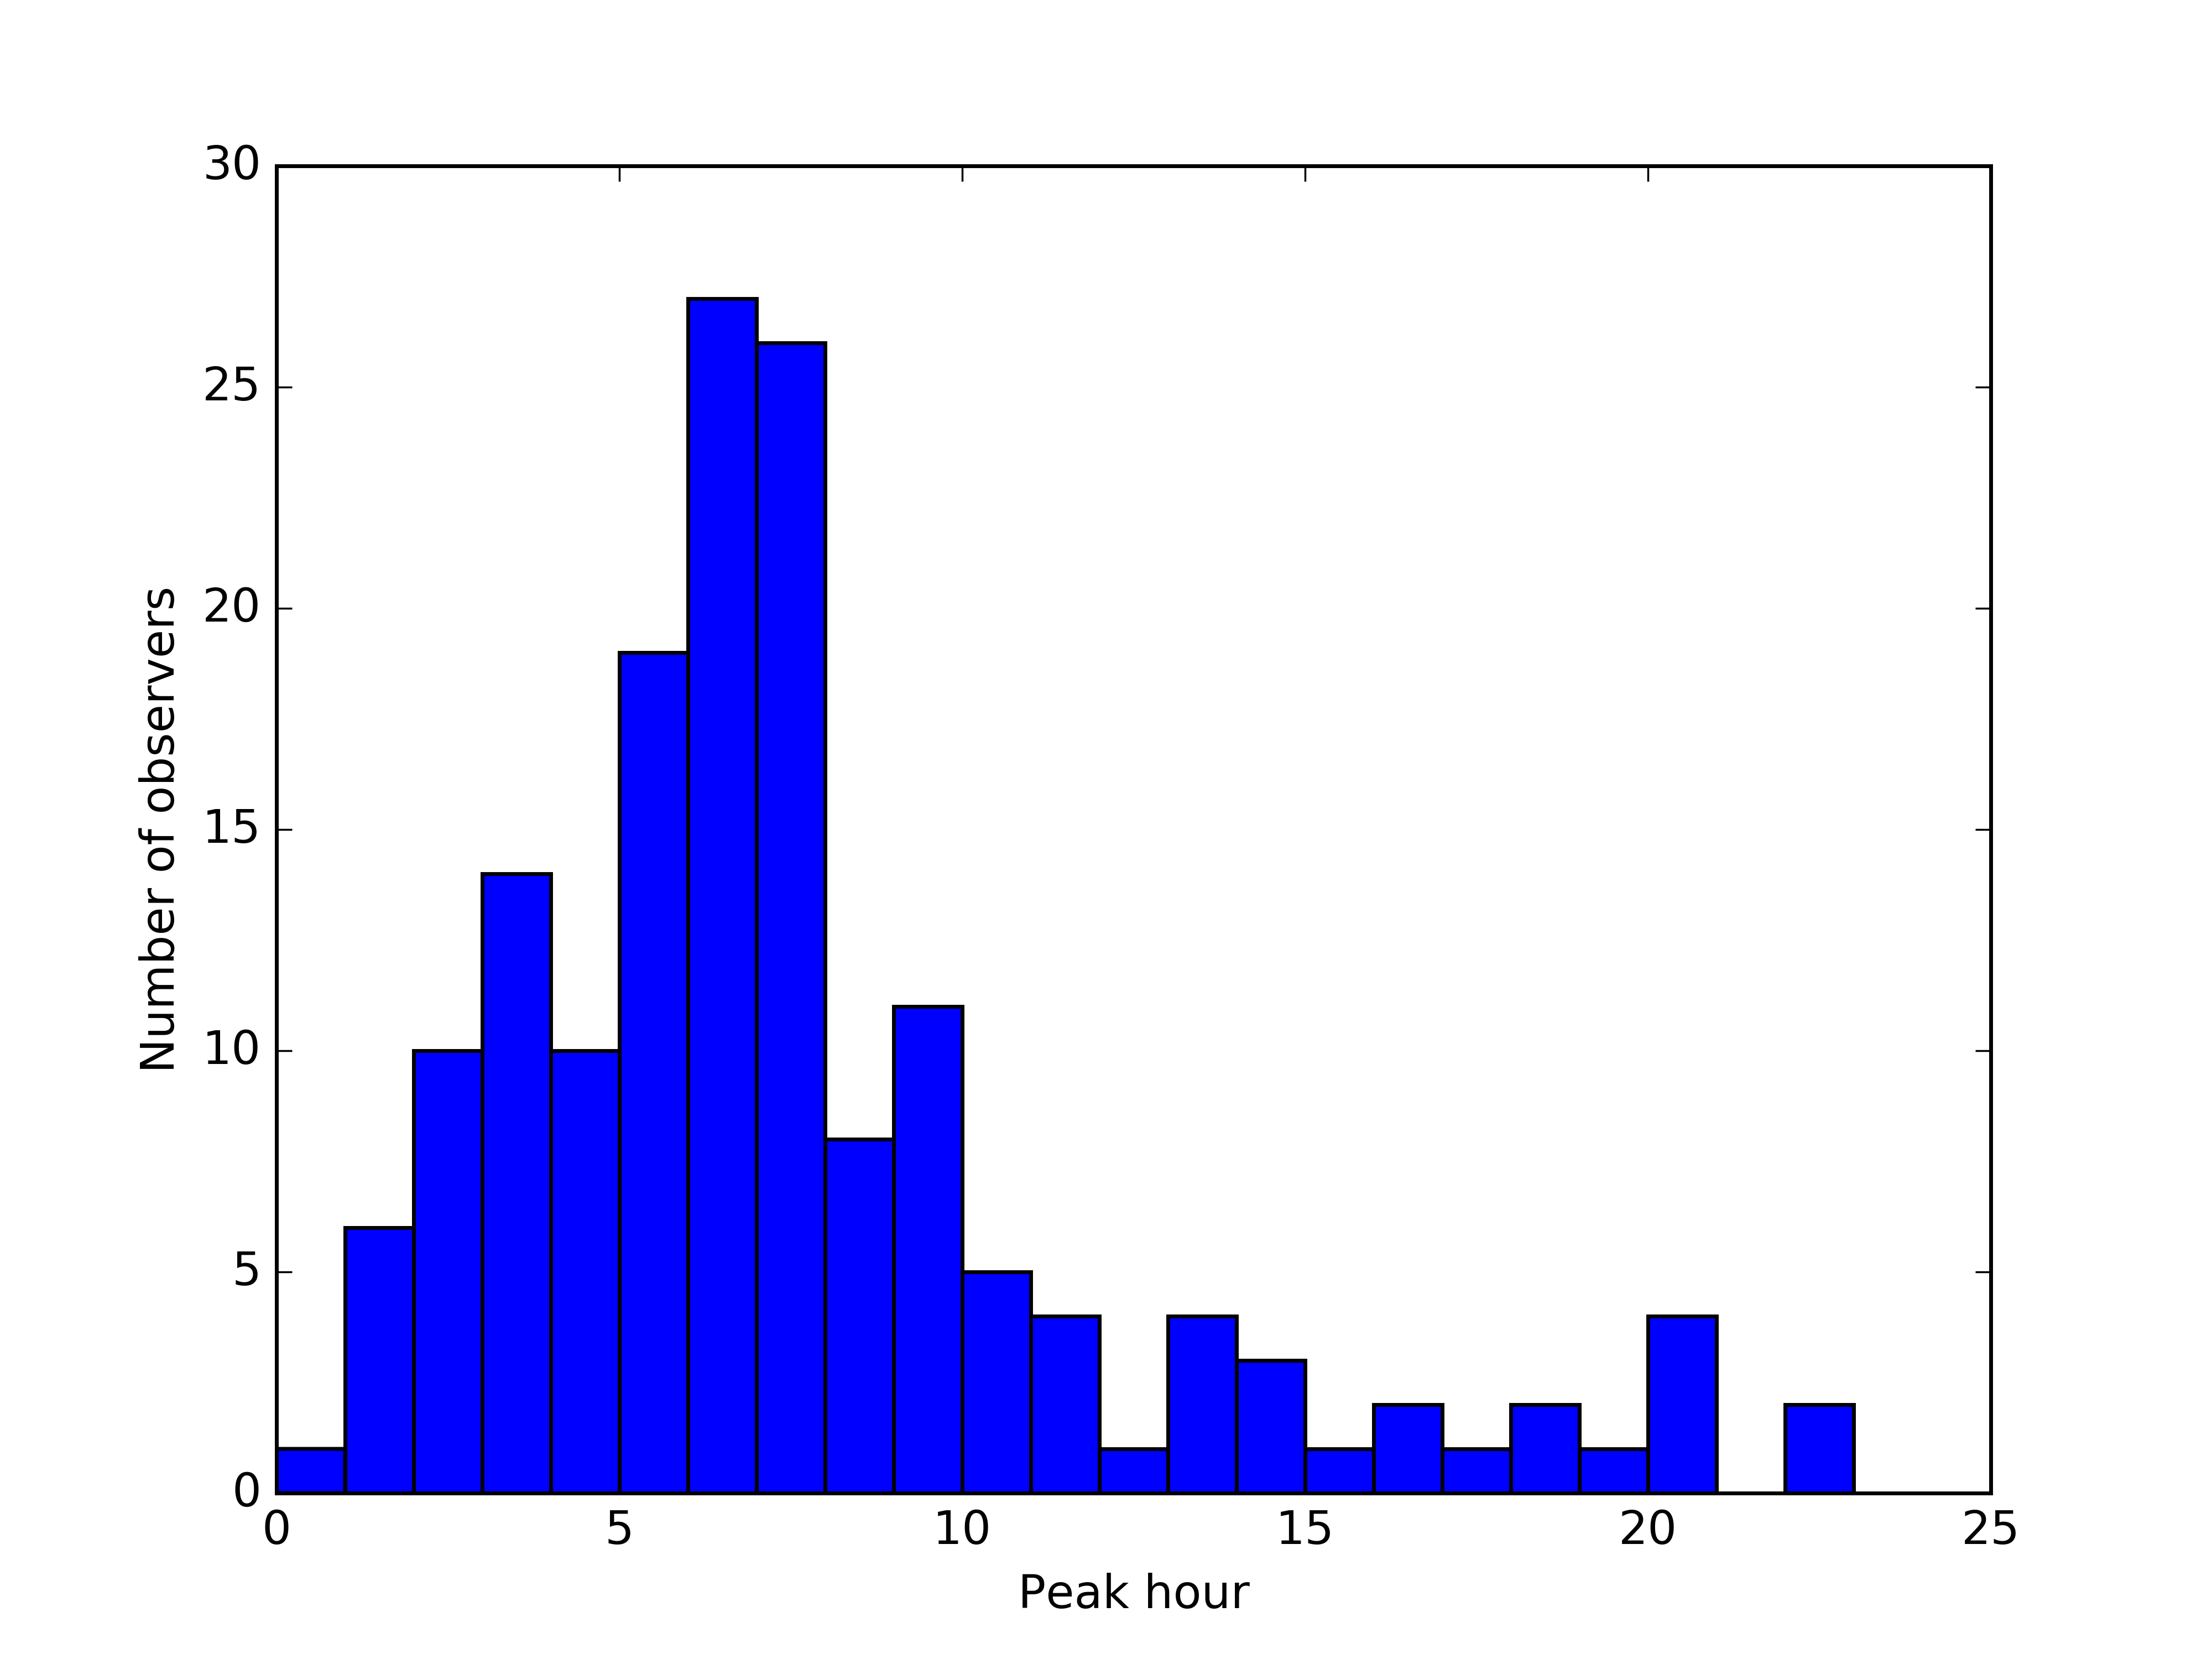
\includegraphics[width=\linewidth]{hist}
	\caption{Histogram of peak hour of diurnal shift in observer's local time \label{fig:hist}}
\end{wrapfigure}

Figure~\ref{fig:hist} shows the peak hour of an observer's apparent diurnal shift in their local time, based on their longitude, not timezones. My model predicts that the peak hour occurs at 6am, and this is seen in the histogram, indicating that my model fits the data. There is some spreading out from this time, as expected by any set of data, though there is also a large number of peak hours at 7am. This is potentially due to changes that occur in the Earth's rotation throughout a year.\\ 

{\large \bf Temporal variation of diurnal shift\\}

Over time, the peak hour of diurnal shift does not appear to increase or decrease, which also supports my model since I provide no reason for the diurnal shift to change with time. Around the time of increased detection rates between 2005 and 2011, diurnal shift appears to be less sinusoidal, indicating an increased background rate, supporting my conclusions from the temporal variation analysis.\\

\end{multicols}
}

%----------------------------------------------------------------------------------------
%	DATA
%----------------------------------------------------------------------------------------

\headerbox{What data am I using?}{name=method,column=0,below=objectives,bottomaligned=conclusion}{ % This block's bottom aligns with the bottom of the conclusion block
\begin{wrapfigure}{r}{0.4\linewidth}
	\centering
	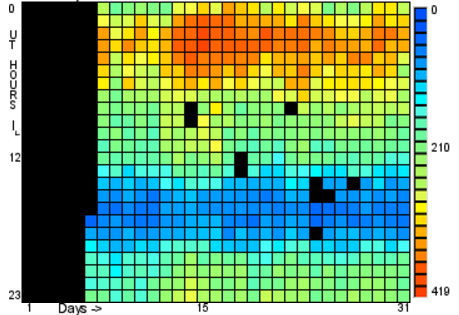
\includegraphics[width=\linewidth]{rmob2}
	\caption{RMOB data in image format \label{fig:rmob}}	
\end{wrapfigure}

For each study I present, the source of my data is the RMOB organisation \cite{rmob}. Started as a group of radio observers hoping to communicate meteor shower results more easily, this group has grown into a worldwide network of radio meteor observation, with each observers' results available for use. The data itself is an hourly detection count. This data is available in one month long sets, as images (figure~\ref{fig:rmob}) or text.\\

\begin{wrapfigure}[10]{r}{0.6\linewidth}
	\centering
	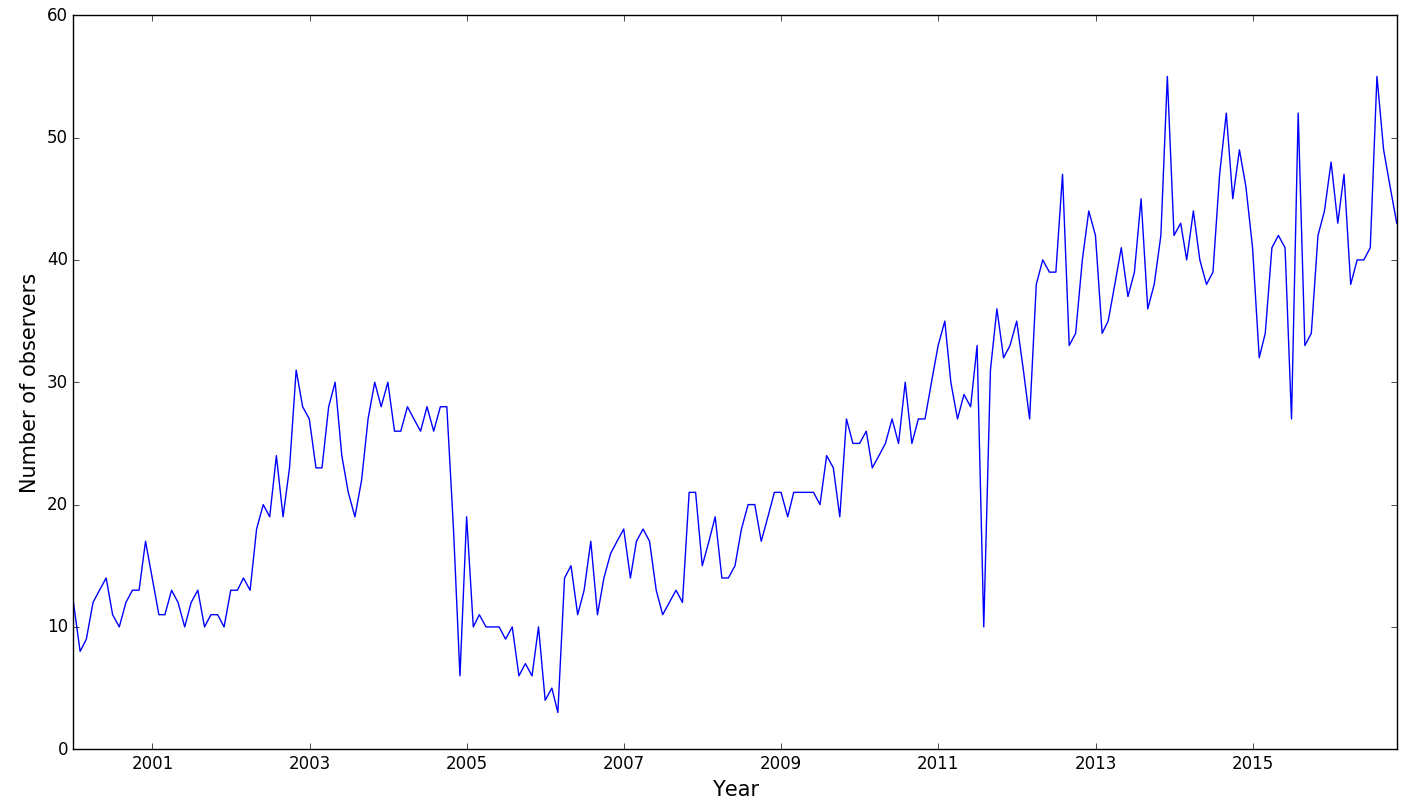
\includegraphics[width=\linewidth]{contributing_authors}
	\caption{Number of observers contributing each month
		\label{fig:contr}}
\end{wrapfigure}

Figure~\ref{fig:contr} shows the number of observers contributing for each month since RMOB text records started. Apart from a sudden drop in 2005, the number of observers is constantly increasing - good news for radio meteor detection analysis! \\
\vspace{2em}

\begin{wrapfigure}[12]{r}{0.75\linewidth}
	\centering
	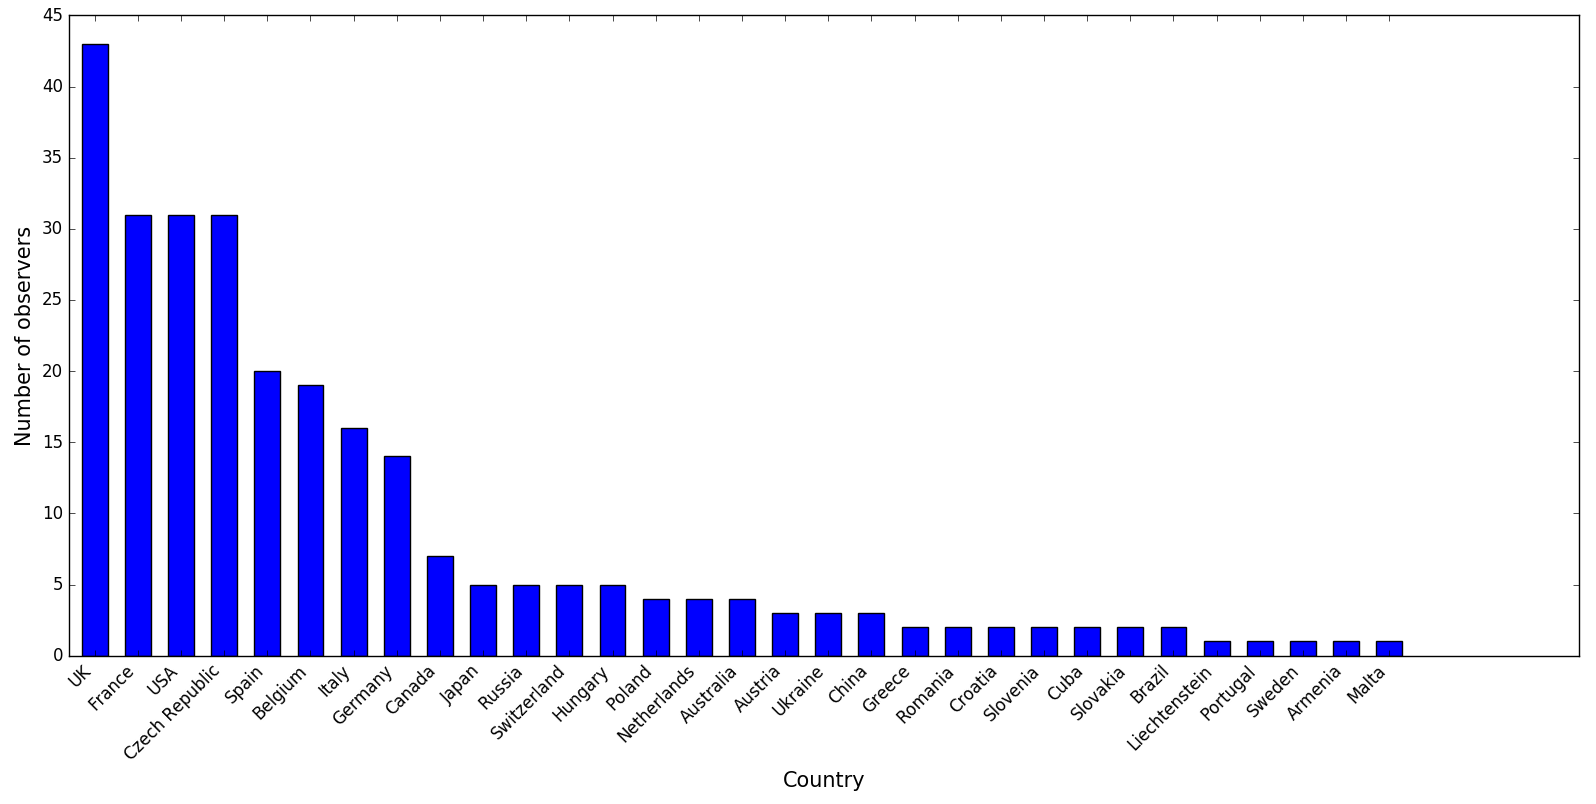
\includegraphics[width=\linewidth]{locations}
	\caption{Locations of observers (where known)
		\label{fig:loc}}
\end{wrapfigure}

Figure~\ref{fig:loc} shows the global reach of the RMOB data. It is clear that most data is from Europe. Overall, there are 3.8 million hourly counts, from 345 observers.\\

}

%----------------------------------------------------------------------------------------
%	ZENITHAL HOURLY RATE
%----------------------------------------------------------------------------------------

\headerbox{Zenithal Hourly Rate}{name=results2,column=1,below=objectives,bottomaligned=conclusion}{ % This block's bottom aligns with the bottom of the conclusion block

{\large \bf Formula}

I have modified the formula for Zenithal Hourly Rate to be used for radio meteor detection. The formula used for visual detection is equation~\ref{eq:vis}, where $F$ is a correction factor for field of view, $r^{6.5-m}$ corrects for the limiting magnitude, and $\overline{HR}$ is the actual visual hourly rate. The equation has a flaw: the $\sin\left( h \right)$ function is used to correct for the height of the radiant (where the meteors `appear' from) above the horizon. This would result in a negative hourly rate with a radiant below the horizon, though meteors are still seen.
\begin{equation}
{ZHR} = \frac{\overline{HR} \cdot F \cdot r^{6.5-{m}}}{\sin \left( h \right)}\label{eq:vis}
\end{equation}
\begin{equation}
{ZHR} = \frac{N - b}{\left( \frac{1}{2} + \frac{h}{\pi} \right)} \label{eq:mine}
\end{equation}
My own correction to this is shown in equation~\ref{eq:mine}, where $b$ is the background hourly rate, $N$ is the actual hourly rate, and $h$ is the angular height of the radiant above the horizon. $F$ and $r^{6.5-m}$ are no longer needed since I assume a field of view covering the whole sky, and the population index model is not valid, since an incredibly large number of meteors would be detected by radios, but aren't.\\

{\large \bf Validity}

In order to test the validity of equation~\ref{eq:mine}, I used it to calculate the theoretical ZHR for 6 common meteors showers for each observer, for years between 2007 and 2016. Most of the results correlate well with the expected visual data. The results do not all have values similar to those expected, though they correlate well since an increase in the visual results is reflected by an increase in radio results -- the offset is likely due to an absent correction factor. In order to determine this, I used the results to calculate a theoretical field of view and limiting magnitude.
The results show that the theoretical limiting magnitude of the antennas used is $\sim 6.75$, and the theoretical field of view is $\sim 30$\%. This field of view should be larger, as should the limiting magnitude. This indicates that there is an offset that is not present as a correction factor. This is expected, however, since I had no data available for field of view and so it was not included. The field of view is highly dependent on the antenna, as is the limiting magnitude.\\

}

%----------------------------------------------------------------------------------------

\end{poster}

\end{document}